\documentclass[11pt]{article}
\PassOptionsToPackage{numbers}{natbib}
% \usepackage[review]{acl}
\usepackage{acl}
\usepackage{times}
\usepackage{latexsym}
\usepackage[T1]{fontenc}
\usepackage[utf8]{inputenc}
\usepackage{microtype}
\usepackage{inconsolata}
\usepackage{graphicx}
\usepackage{amsmath}
\usepackage{amssymb}
\usepackage{algorithm}
\usepackage{algorithmic}
\usepackage[textsize=tiny,backgroundcolor=pink]{todonotes}
\usepackage{caption}
\usepackage{placeins}
\usepackage[most]{tcolorbox}
\usepackage{titletoc}

\title{QueryBloom: Automated Text-SPARQL Example Synthesis via Subgraph Sampling}

\author{Essam Wisam \and Chengkai Li \\
  The University of Texas at Arlington \\
  Arlington, TX, USA \\
  \texttt{\{abdelghanye, cli\}@uta.edu}}

\begin{document}
\maketitle

\begin{abstract}
Text-SPARQL example sets are indispensable for training, tuning, and evaluating Knowledge Graph Question Answering (KGQA) systems, yet they remain scarce for various knowledge graphs due to the extent of manual effort required. We present \textit{QueryBloom}, an automated, KG-agnostic methodology that synthesizes diverse, comprehensive and high-quality Text-SPARQL examples requiring only a SPARQL endpoint for the target knowledge graph. The approach systematically samples structurally diverse multi-hop subgraphs from the knowledge graph, before employing an LLM-driven multi-agent framework to synthesize grounded text--SPARQL pairs and progressively refine them for complexity, correctness, and fluency. Evaluation against the human-authored DBpedia QALD-9 benchmark demonstrates that QueryBloom matches or exceeds established benchmarks in query structural complexity, semantic linguistic variety, and schema coverage.
\end{abstract}

\section{Introduction}
\label{sec:introduction}
RDF knowledge graphs (KGs) have become a standard framework for structuring open-domain information, as exemplified by knowledge bases such as DBpedia and Wikidata \cite{auer2007dbpedia, vrandecic2014wikidata}. Simultaneously, their application has expanded to capture complex, domain-specific knowledge in areas ranging from soil carbon and climate modeling to medicine and sociology \cite{frink_proto-okn}. SPARQL has become the standard query language for RDF knowledge graphs, with hundreds of queryable endpoints emerging since its inception \cite{ali2022survey}. Owing to the technical barrier of composing SPARQL queries, Knowledge Graph Question Answering (KGQA) systems have become essential for democratizing access to knowledge graphs, enabling researchers, domain-experts, and ordinary users to seamlessly reason about such knowledge by mapping natural language questions to SPARQL queries that can be executed against the graph to provide accurate answers. 
% Crucially, these systems guard against model hallucinations in an era where large language models are the primary front-end for information access.
\todo{discussing KGQA in the context of Ai.}\todo[color=green]{the users are not just researchers. it could be domain experts, non experts, and agentic systems too.}\todo[color=green]{make it more convincing and explicit that SPARQL is still crucial.}

Text-SPARQL example sets play a central role for KGQA systems.\todo[color=cyan]{More systematic exploration of the distinction between 3 natural language query formats: keywords, questions, and commands.} They serve as in-context demonstrations that steer LLM-based query generation \cite{wikisp2023,zahera2024generating, dabramo-etal-2025-investigating,emonet2024llm}, as training corpora for fine-tuning translation models \cite{sgpt2022generative,neural2022machine}, and as standardized benchmarks for measuring system correctness \cite{dubey2019lcquad, usbeck2019qald,usbeck2021qald}. Beyond training and evaluation, these example sets are often used as executable documentation, helping human practitioners better navigate unfamiliar knowledge graph structures and query idioms \cite{uniprot_sparql_examples, wikidata_sparql_examples}.

Constructing high-quality Text-SPARQL example sets for a given knowledge graph is a costly and time-consuming process because it requires three distinct areas of expertise: (i) fluency in the specific target domain, (ii) proficiency in formal SPARQL query construction, and (iii) a deep familiarity with the knowledge graph's ontology, including its semantics, structure, and vocabulary. Existing curated Text-SPARQL benchmarks concentrate on a handful of prominent open-domain knowledge graphs, principally DBpedia, Wikidata, and Freebase, and rely on manual question authoring, template-based construction, and contributions from the open-source community \cite{usbeck2019qald,usbeck2021qald,trivedi2017lc,dubey2019lcquad,wikisp2023,liu2024spinach}.\todo[color=green]{Make it clear that QALD and so on are such existing benchmarks on open-domain KGs.}\todo[color=green]{Unclear why we discuss each benchmark's creation} Domain-specific knowledge graphs, which encode specialized knowledge in fields such as biomedicine \cite{kgs2025biomedical}, geoscience \cite{sockg2025}, and climate models \cite{adamu2025climatepub4kg}, lack equivalent community infrastructure and consequently have few or no Text-SPARQL resources \cite{frink_proto-okn}. This scarcity has confined the majority of KGQA research \cite{liu2024spinach,zahera2024generating,sgpt2022generative,kacupaj2023sparqlgen,banerjee2022modern,diallo2025frase,sun2022think,wikisp2023} to the open-domain settings where Text-SPARQL example sets already exist, leaving domain-specific settings largely unaddressed, and depriving domain researchers of the automated QA interfaces necessary to seamlessly reason over specialized knowledge embedded in domain-specific knowledge graphs.

To address this gap, there is a need for an automated KG-agnostic methodology that can generate reliable, diverse and comprehensive Text-SPARQL pairs for arbitrary knowledge graphs, which to the best of our knowledge no prior work has yet addressed. To bridge this gap, we present QueryBloom, an automated, KG-agnostic methodology that can synthesize high-quality Text-SPARQL example sets from any RDFS-based knowledge graph given only SPARQL endpoint access.\todo[color=green]{Need to articulate the motivations behind the methodology design before you detail the methods.} The approach is motivated by the two following observations: (i), it is possible to discover arbitrary subgraph patterns for any given RDFS-based knowledge graph using KG-agnostic RDFS-based exploration queries (Subgraph Discoverability) and (ii), every SPARQL query implicitly specifies a subgraph pattern over the knowledge graph (SPARQL-Subgraph Duality). QueryBloom inverts the duality by using an LLM agentic pipeline to generate Text-SPARQL queries grounded on subgraph instances and patterns automatically discovered from the target knowledge graph.

Concretely, the QueryBloom pipeline proceeds in four stages: (1) extracting one-hop subgraph type patterns encoding which properties connect which types of entities; (2) growing a set of structurally diverse multi-hop subgraphs by iteratively extending seed patterns through adjacency-guided attachment; (3) enriching each subgraph with concrete entity instances and attribute values; and (4) employing an agentic pipeline that filters non-meaningful subgraphs, jointly generates natural language questions and SPARQL queries, augments the pairs to introduce meaningful complexity, iteratively verifies each pair against the endpoint, and finally refines phrasing for the generated questions.

\todo{Explain the evaluation, summarize the results, and other aspects before the ``summary''.}

In summary, our key contributions are as follows:\todo[color=green]{can have more bullet points.}
\begin{itemize}
	\item QueryBloom, an LLM-driven methodology that synthesizes diverse, accurate and, comprehensive Text-SPARQL examples for a target knowledge graph given only its SPARQL endpoint. It tackles the example scarcity challenge for domain-specific knowledge graphs and facilitates
 the development of their KGQA systems.
	\item A comprehensive evaluation framework demonstrating that QueryBloom-generated datasets match or exceed the diversity of established human-authored benchmarks across query structural complexity, semantic linguistic variety, and holistic schema coverage.
	\item Three novel Text-to-SPARQL datasets across diverse domain scopes: open-domain (\textsc{DBpedia}), broad-domain (\textsc{DBLP}), and domain-specific (\textsc{SOCKG}).
\end{itemize}
\section{Related Work}
\label{sec:related}

\todo[color=green]{Are there related work in terms of methodology?}

\textbf{Text-SPARQL Datasets.} Several curated benchmarks have driven progress in KGQA. The QALD challenge series~\cite{usbeck2019qald,usbeck2021qald} provides hand-crafted questions over DBpedia and Wikidata, while LC-QuAD~\cite{trivedi2017lc} and LC-QuAD 2.0~\cite{dubey2019lcquad} use template-based generation with human paraphrasing to scale dataset size. WikiSP~\cite{wikisp2023} sources questions from search logs to better reflect real user information needs. Spinach~\cite{liu2024spinach} curates questions from Wikidata's ``Request a Query'' forum, capturing authentic complexity beyond synthetic benchmarks. All of these resources target open-domain knowledge graphs such as Wikidata, DBpedia, and Freebase; domain-specific graphs, which lack equivalent breadth or community efforts, have no comparable Text-SPARQL coverage. \todo[color=green]{It seems obvious that they cannot be transferred.}

\textbf{KGQA via NL-SPARQL Translation.} KGQA has seen significant advances with the emergence of Large Language Models (LLMs), which have achieved state-of-the-art performance compared to prior deep learning and classical approaches \cite{dabramo-etal-2025-investigating,sgpt2022generative}. LLM-based approaches include chain-of-thought prompting for SPARQL generation \cite{zahera2024generating}, fine-tuning on text-SPARQL pairs \cite{sgpt2022generative,neural2022machine}, and in-context learning with retrieved examples \cite{emonet2024llm}. Agentic approaches such as GRASP~\cite{walter2025grasp} and Spinach~\cite{liu2024spinach} employ LLMs with tool-use for interactive graph exploration.\todo[color=green]{you mentioned these are not fully accurate.} All of these approache require or at least benefit from Text-SPARQL examples. QueryBloom is thus, complementary to these systems, as it can automatically provide the example sets they require for arbitrary RDFS-based knowledge graphs.

\textbf{Synthetic Data Generation.} Template-based approaches such as LC-QuAD~\cite{trivedi2017lc} generate questions from fixed SPARQL templates, but require manual template design per knowledge graph. Labate et al.~\cite{labate2025synthetic} recently proposed using LLMs to replace crowdsourced paraphrasing of LC-QuAD's template-generated questions, showing that synthetic rephrasings can match human quality for fine-tuning; however, their method still depends on LC-QuAD's existing template infrastructure and is limited to Wikidata. Deviating from template-based generation, KGQAGen~\cite{zhang2025kgqagen}, employs LLMs to generate at most one Wikidata-specific Text-SPARQL pair for each seed entity drawn from Wikipedia vital articles with the aim of improving factual quality issues observed in earlier benchmarks. While similar to QueryBloom in generating the Text-SPARQL pairs grounded on knowledge embedded in the graph, their method is designed specifically for Wikidata and uses Wikidata-specific APIs. Moreover, it generates questions strictly bounded by the number of seed entities given. In contrast, QueryBloom is designed to be applicable on any RDFS-based knowledge graph given its SPARQL endpoint and comprehensively generates Text-SPARQL pairs covering the schema underlying the knowledge graph while optionally requiring a single seed for the whole knowledge graph. The two methods could be viewed as complementary because Wikidata does not follow the RDFS standard required by QueryBloom and offers various resources, including seed entities and APIs, that make KGQAGen possible. In contrast, QueryBloom is designed to operate on any RDFS-based knowledge graph and does not assume access to such specific resources.
\section{Methodology}
\label{sec:methodology}

\begin{figure}[t]
	\centering
	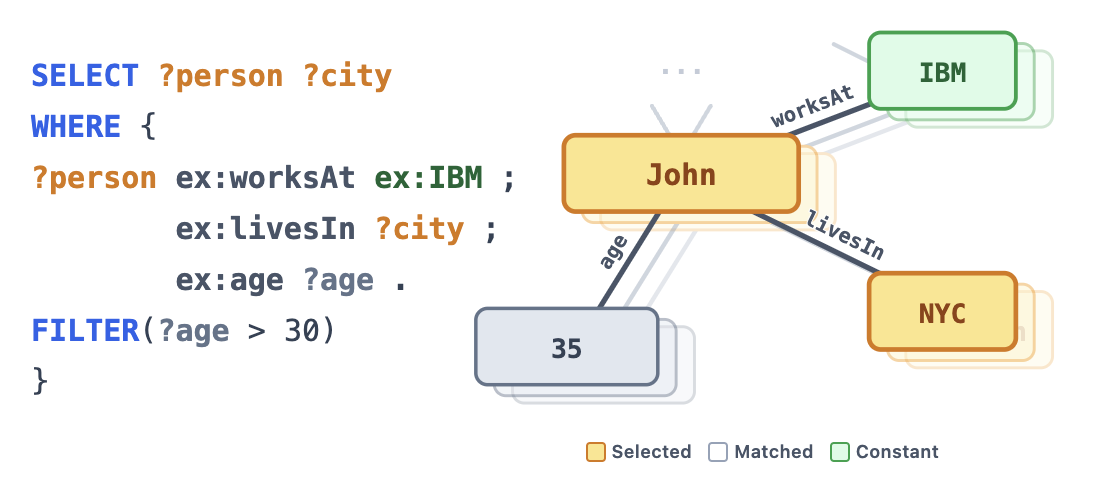
\includegraphics[width=\columnwidth]{figures/sparql.png}
	\captionsetup{skip=4pt}
	\caption{Correspondence between a SPARQL query and its matched knowledge graph subgraph.}
	\label{fig:sparql-subgraph}
\end{figure}

The central observation underlying QueryBloom is that every SPARQL query implicitly specifies a subgraph pattern over the knowledge graph (Figure~\ref{fig:sparql-subgraph}). The triple patterns in a \texttt{WHERE} clause define nodes and labeled edges that must be matched in the graph, while \texttt{SELECT} projects specific variables, and \texttt{FILTER} imposes value constraints. Each returned result row corresponds to a distinct embedding of this pattern in the graph data: a concrete assignment of entities to the query's variables that satisfies all structural and value constraints. The same argument applies to other SPARQL query forms (\texttt{ASK}, \texttt{CONSTRUCT}), which rely on the same \texttt{WHERE} clause pattern matching mechanism.

QueryBloom inverts this correspondence: it first discovers structurally diverse subgraph patterns from the knowledge graph and then jointly synthesizes SPARQL queries and natural language questions grounded in those patterns (Figure~\ref{fig:querybloom-pipeline}).

\begin{figure}[t]
	\centering
	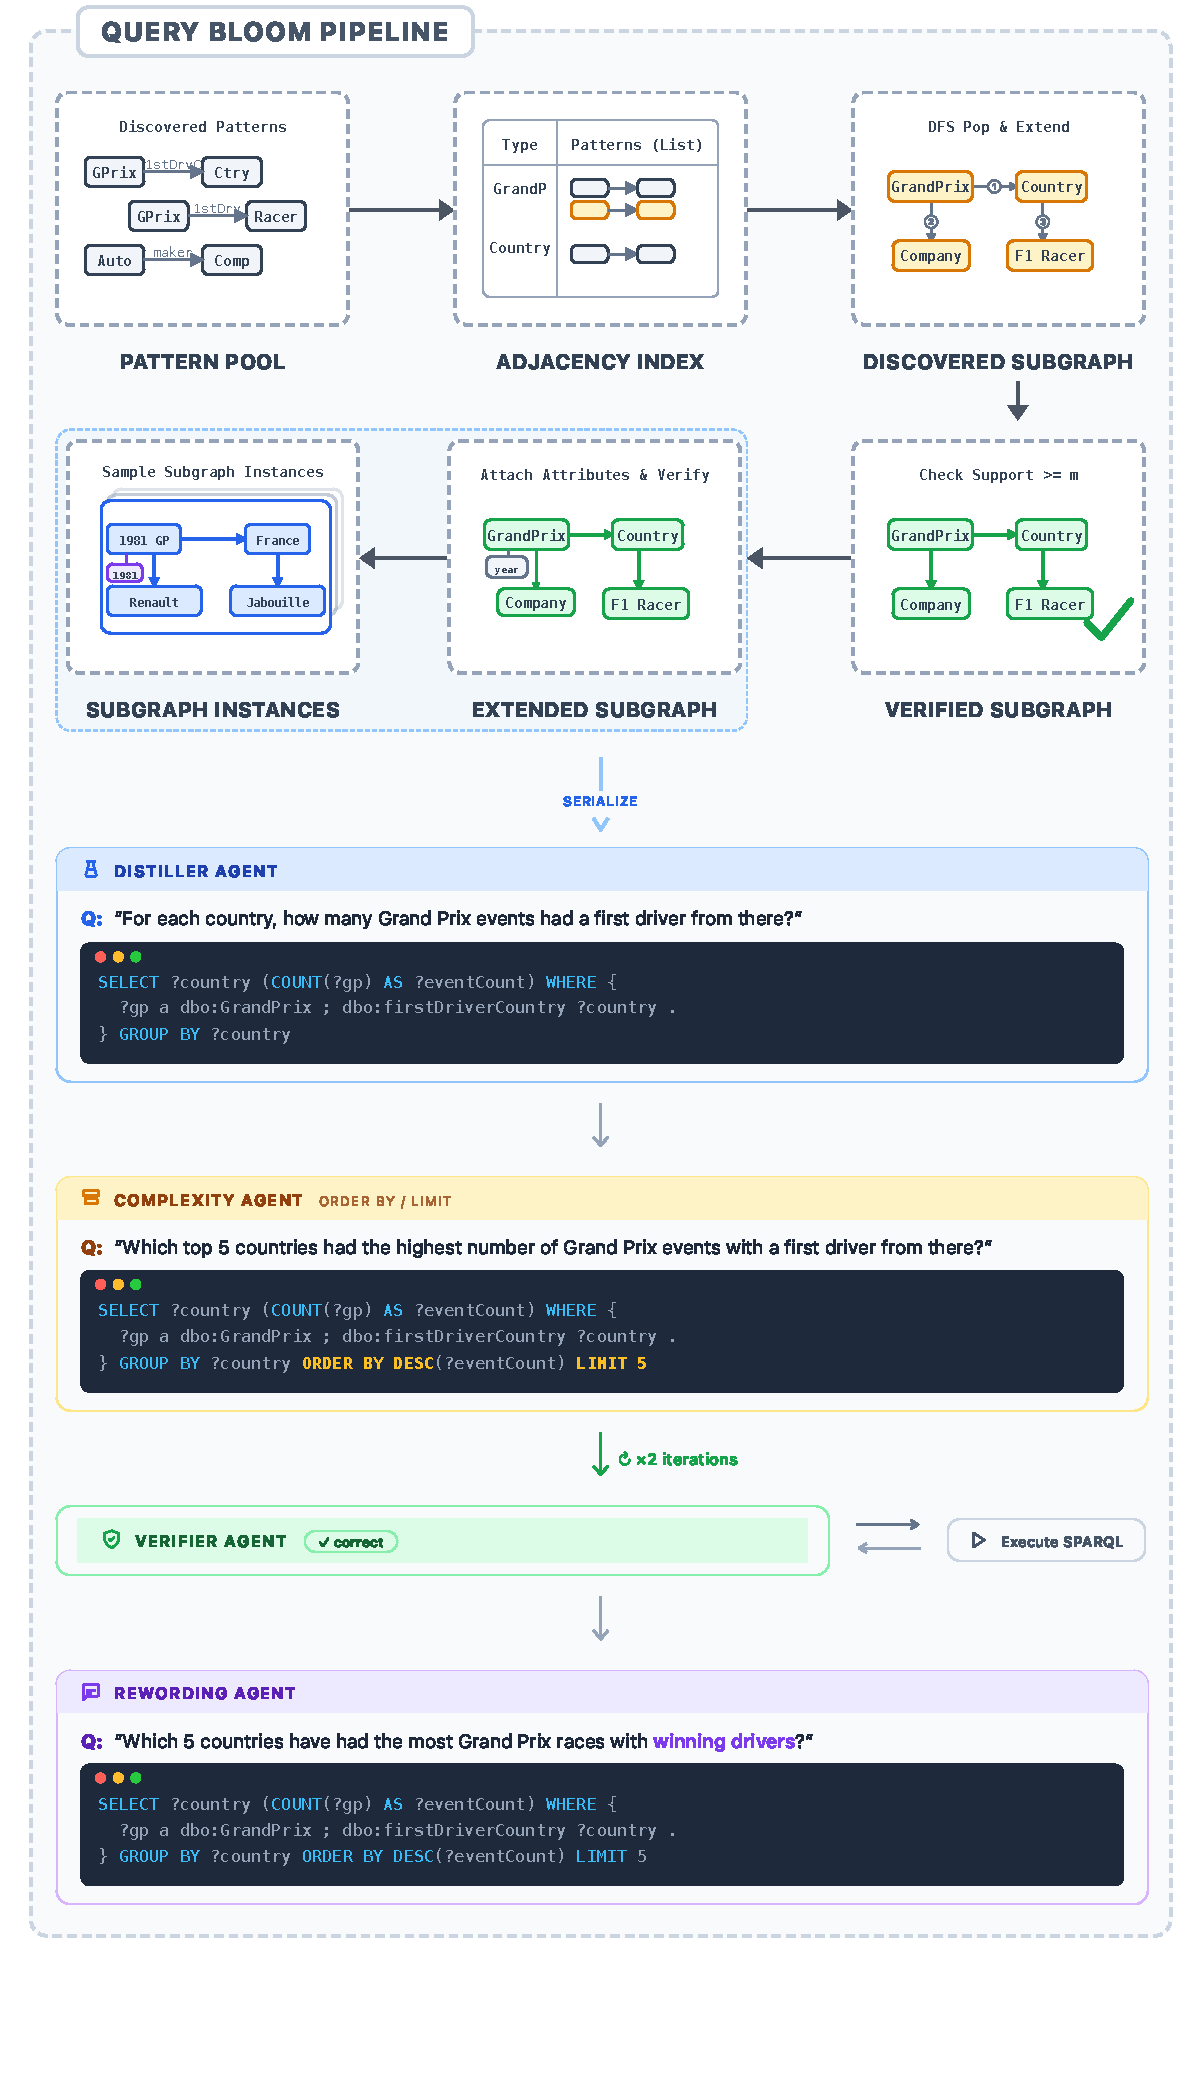
\includegraphics[width=\columnwidth,trim=0 70bp 0 0,clip]{figures/QB-Col.pdf}
	\captionsetup{skip=4pt}
	\caption{Overview of the QueryBloom methodology.}
	\label{fig:querybloom-pipeline}
\end{figure}

The pipeline proceeds through the multiple stages described below, which trace how a single subgraph pattern is discovered, grounded, and distilled into a small set of text-SPARQL pairs. The framework relies on the minimal assumption that the target knowledge graph follows W3C RDFS standards for defining classes, which is a common practice in almost all RDF knowledge graphs.

\subsection{Pattern Discovery and Adjacency Indexing}

The pipeline begins by extracting \textit{frequent type patterns} from a
property scope chosen for the target knowledge graph, adapting the ABSTAT
algorithm~\cite{Spahiu2016ABSTATOL} for efficient pattern extraction over RDF
graphs. A type pattern is a triple $(\textit{SubjectType},\;\textit{Predicate},
\;\textit{ObjectType})$ encoding that a given property connects instances of one
type to instances of another (e.g., \texttt{Person} --\texttt{worksAt} --\texttt{Organization}); patterns are discovered by sampling a large set of
triples for each property and resolving the \texttt{rdf:type} of their subject
and object nodes.

QueryBloom supports two preprocessing modes that differ in how the property
scope is determined. \textit{Whole-graph mode}, suited to smaller knowledge
graphs, enumerates all properties via a SPARQL query, removes common metadata
predicates such as labels and identifiers, and extracts patterns from the
resulting set. \textit{Online-graph mode}, suited to large graphs, begins from a
single user-specified seed property, extracts its type patterns, and then
iteratively selects properties connected to already-discovered types, adding
their patterns until a configurable property budget is reached.

In both modes, the collected patterns are filtered by a minimum support
threshold $\sigma$; the resulting set of patterns form the structural building blocks for
subgraph construction. An adjacency index is then built over this pool, mapping
each type to every pattern in which it participates and enabling constant-time
lookup of candidate extensions during subgraph discovery.

\subsection{Subgraph Discovery}

A multi-hop subgraph pattern is grown from a single frequent pattern, which serves as a two-type seed. The seed is iteratively extended by attaching adjacent patterns from the adjacency index that share at least one type with the current subgraph. Each extension adds a new edge and may introduce new types, continuing until a subgraph with $k$ distinct types is formed. At each extension, the subgraph's support is verified via a SPARQL \texttt{COUNT} query and the extension is discarded if it causes the subgraph's support to fall below the threshold $\sigma$. It follows that the subgraph will contain at least $k-1$ properties and may be cyclic or acyclic.

Once a k-type subgraph is formed, it is enriched in two further steps. First, data attributes are sampled from the discovered attribute patterns and attached to the subgraph's types and verified. Second, $m$ concrete entity instances per type that jointly satisfy the subgraph's type and property constraints are fetched from the endpoint, along with their attribute values. The subgraph comprises the abstract subgraph pattern and grounding instances with real entity URIs, labels, and attribute values to inform realistic question generation.


\subsection{LLM-Driven Text-SPARQL Distillation}

Each verified subgraph is processed by a four-stage multi-agent system whose collective purpose is to distill the subgraph into a small set of high-quality, execution-verified text-SPARQL pairs. The four agents — a \textit{generator}, a \textit{complexity introducer}, a \textit{verifier}, and a \textit{reword auditor} — operate in sequence, each receiving the subgraph as a structured YAML representation. All agents use structured output with enforced JSON schemas to guarantee perfectly parseable responses \cite{openai2024structured}.

\paragraph{Generation.}
The generator agent first assesses whether the subgraph pattern admits meaningful questions about the knowledge graph, exiting early if not. If meaningful, it generates a set of text-SPARQL pairs grounded in the subgraph's classes, entities, relationships, and attributes (see Appendix~\ref{sec:appendix_prompt}). Each generated SPARQL query is immediately executed against the endpoint, and its results are recorded alongside the pair.

\paragraph{Complexity Introduction.}
To ensure that generated question–query pairs match the complexity of real-world examples, a
\textit{complexity introducer} agent rewrites each successfully executed pair to meaningfully incorporate
additional non-trivial constructs drawn from a predefined set: value filtering, optional matching,
set union, sorting and limiting, existential checks, nested subqueries, and recursive relationships. Both the SPARQL query and its corresponding natural language question are rewritten
consistently to reflect the introduced construct. Where no meaningful augmentation is possible,
the agent skips the pair and retains the original. Every augmented query is re-executed against
the endpoint to update the execution results.

\paragraph{Verification.}
Although grounding generation in a concrete subgraph pattern is in principle sufficient to produce accurate text-SPARQL pairs (Section~\ref{sec:methodology}), an LLM is still prone to hallucination or innovation while forming the text-SPARQL. An iterative verifier agent therefore inspects every pair. Given the subgraph pattern and each pair's question, query, and execution results, the verifier judges each pair as \textit{correct} or \textit{needs-fix}. For pairs it deems in need of fixing, it additionally produces corrected question and query texts; the corrected queries are re-executed and the updated pairs are fed back into the next verification round. The loop runs for up to a configurable number of iterations or until all pairs are marked correct.

\paragraph{Question Rewording.}
As a final step, a reword agent audits the natural language question of each correct pair for KG-specific terminology leakage — such as exposed URI fragments, ontology class names, or other non-natural phrasings — and rewrites only the question text of flagged pairs, leaving the SPARQL query unchanged.

All four LLM calls operate with high reasoning effort to maximise correctness, and only pairs that pass verification are retained in the final dataset.

\subsection{Design Principles}

The pipeline is designed to produce a text-SPARQL example set that is \textit{comprehensive}, \textit{diverse}, and of \textit{high quality}.

\paragraph{Comprehensiveness.} The overall algorithm orchestrates the stages described above by seeding at least one subgraph from every frequent type pattern in the constructed pool. Thus, coverage is defined with respect to the chosen preprocessing mode: whole-graph mode covers all frequent patterns found among the graph's selected non-metadata properties, whereas online graph mode covers all frequent patterns found for the seed property and any connected properties added within the property budget. As opposed to graph mining, we deliberately adopt a very low support threshold because even rare subgraph patterns can give rise to meaningful questions.


\paragraph{Diversity.} Several mechanisms ensure diversity in the generated examples: (i) unlike a random walk that follows a linear path, the subgraph is extended by selecting a new pattern from \textit{any type} contained in the current subgraph, producing diverse structural compositions; (ii) the target number of types $k$ is sampled from a range distribution to produce subgraphs of varying sizes; (iii) for each subgraph, we randomly sample $v$ attributes per class to ensure diverse coverage of class attributes; (iv) the distiller agent is prompted to produce variations in question and query style, covering different query patterns (e.g., \texttt{SELECT}, aggregation, \texttt{ASK}, \texttt{FILTER}, \texttt{OPTIONAL}, \texttt{GROUP BY}).

\paragraph{Quality.} Quality is safeguarded at multiple stages. Subgraphs that are trivial or concern only graph metadata are flagged as non-meaningful during generation and excluded. The generate-execute-verify loop ensures that every retained pair produces results expected by the distiller agent. The distiller agent's core objective is to elicit questions from the subgraph that a domain expert would be expected to ask.

\FloatBarrier
\section{Results}
\label{sec:evaluation}

\subsection{Dataset Quality and Diversity}

\FloatBarrier

To assess the quality and structural diversity of datasets generated by QueryBloom, we compare a synthesized dataset against DBpedia QALD-9, a standard human-authored benchmark. We evaluate diversity across three dimensions: query feature complexity, semantic linguistic variety, and holistic schema coverage.


\textbf{Query Structural Complexity.} The distribution of SPARQL 1.1 operators within both datasets shows that QueryBloom demonstrates significantly higher structural complexity in several key dimensions compared to the QALD-9 baseline. Notably, QueryBloom queries incorporate \texttt{FILTER} constraints at roughly four times the rate of the baseline. Furthermore, they heavily utilize \texttt{OPTIONAL} blocks and property paths, which are entirely absent from the QALD-9 test set. Both datasets maintain a comparable usage of \texttt{UNION} operators. This confirms that QueryBloom maintains a higher level of structural complexity than the QALD-9 baseline which more closely reflects the complexity of real-world SPARQL queries.

\textbf{Semantic Linguistic Diversity.} To evaluate the natural language variety of the generated questions, we compute dense semantic embeddings for each question text using SBERT (BGE-large) and project these embeddings into a 2D space via t-SNE. We compute Average Pairwise Distance (APD) for global diversity and Mean Nearest-Neighbour Distance (MNND) for local density. QueryBloom achieves a higher APD and MNND, which indicates that QueryBloom successfully covers a wider semantic space of linguistic intents and vocabulary than the fixed human-authored QALD-9 test set.

\textbf{Holistic Schema Coverage.} We present a multi-dimensional summary of dataset diversity across five key metrics:
\begin{itemize}
    \item \textbf{Unique Entities \& Relations:} The average number of distinct entities and properties referenced per query, reflecting how broadly the dataset explores the underlying knowledge graph schema.
    \item \textbf{Variables \& Triples:} The median number of variables and triple patterns per query, measuring the structural size and depth of the generated SPARQL.
    \item \textbf{Unique Templates:} The ratio of distinct SPARQL skeletons (where specific entities, variables, and literals are anonymized) to the total number of queries, assessing syntactic novelty.
\end{itemize}

QueryBloom outperforms QALD-9 across almost all these dimensions. Most strikingly, it achieves a substantially higher unique template ratio, indicating that its SPARQL skeletons are even more diverse than those found in the human-authored benchmark. The next clearest difference is structural depth, with QueryBloom producing a median of roughly three times as many triple patterns per query as the baseline. Furthermore, it consistently incorporates a higher rate of unique entities per query, ensuring broader and more diverse coverage of the graph's instance data.

\begin{figure*}[p]
    \centering
    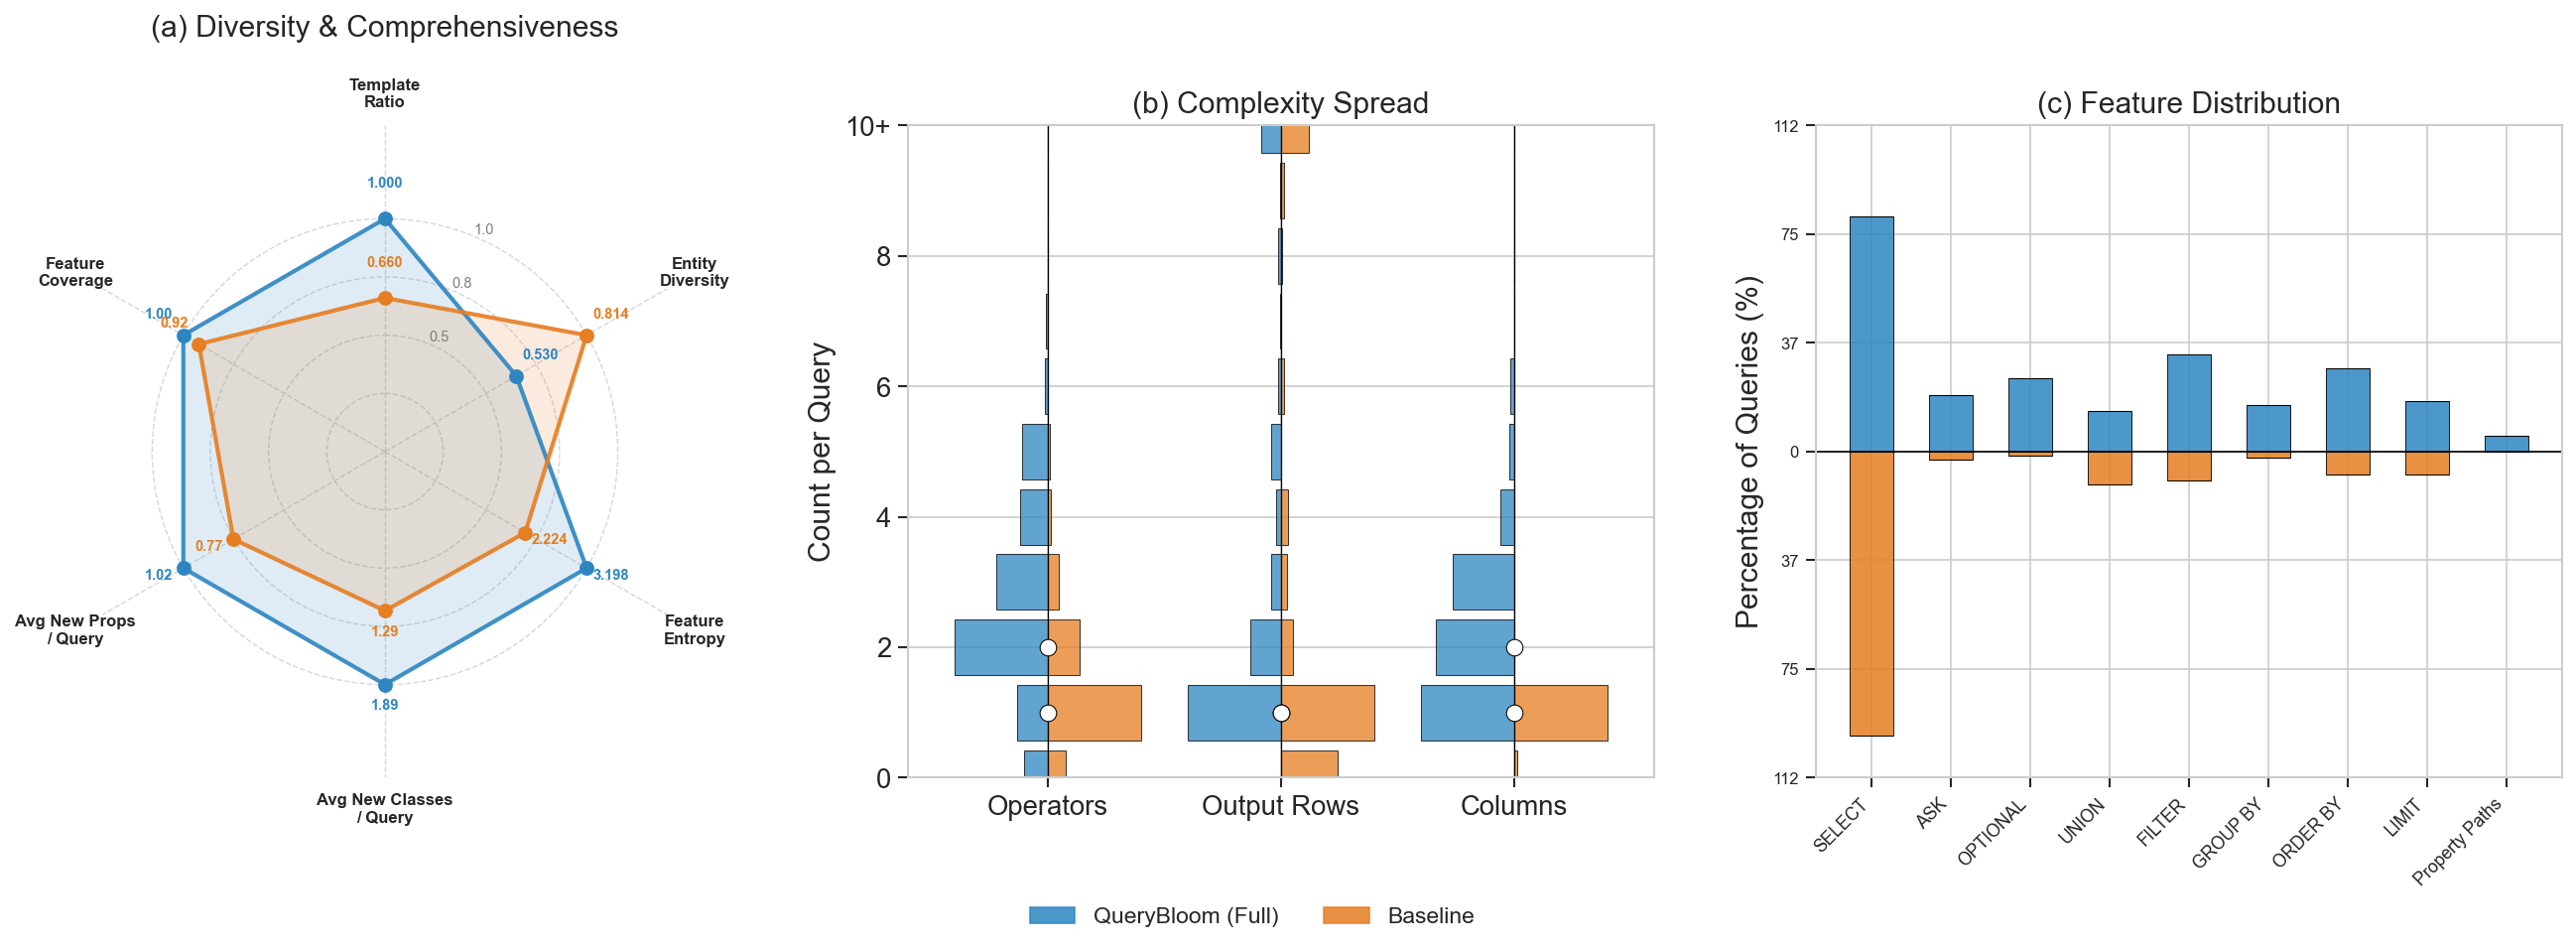
\includegraphics[width=\textwidth]{figures/eval/diversity-dbpedia.png}
    \par\medskip
    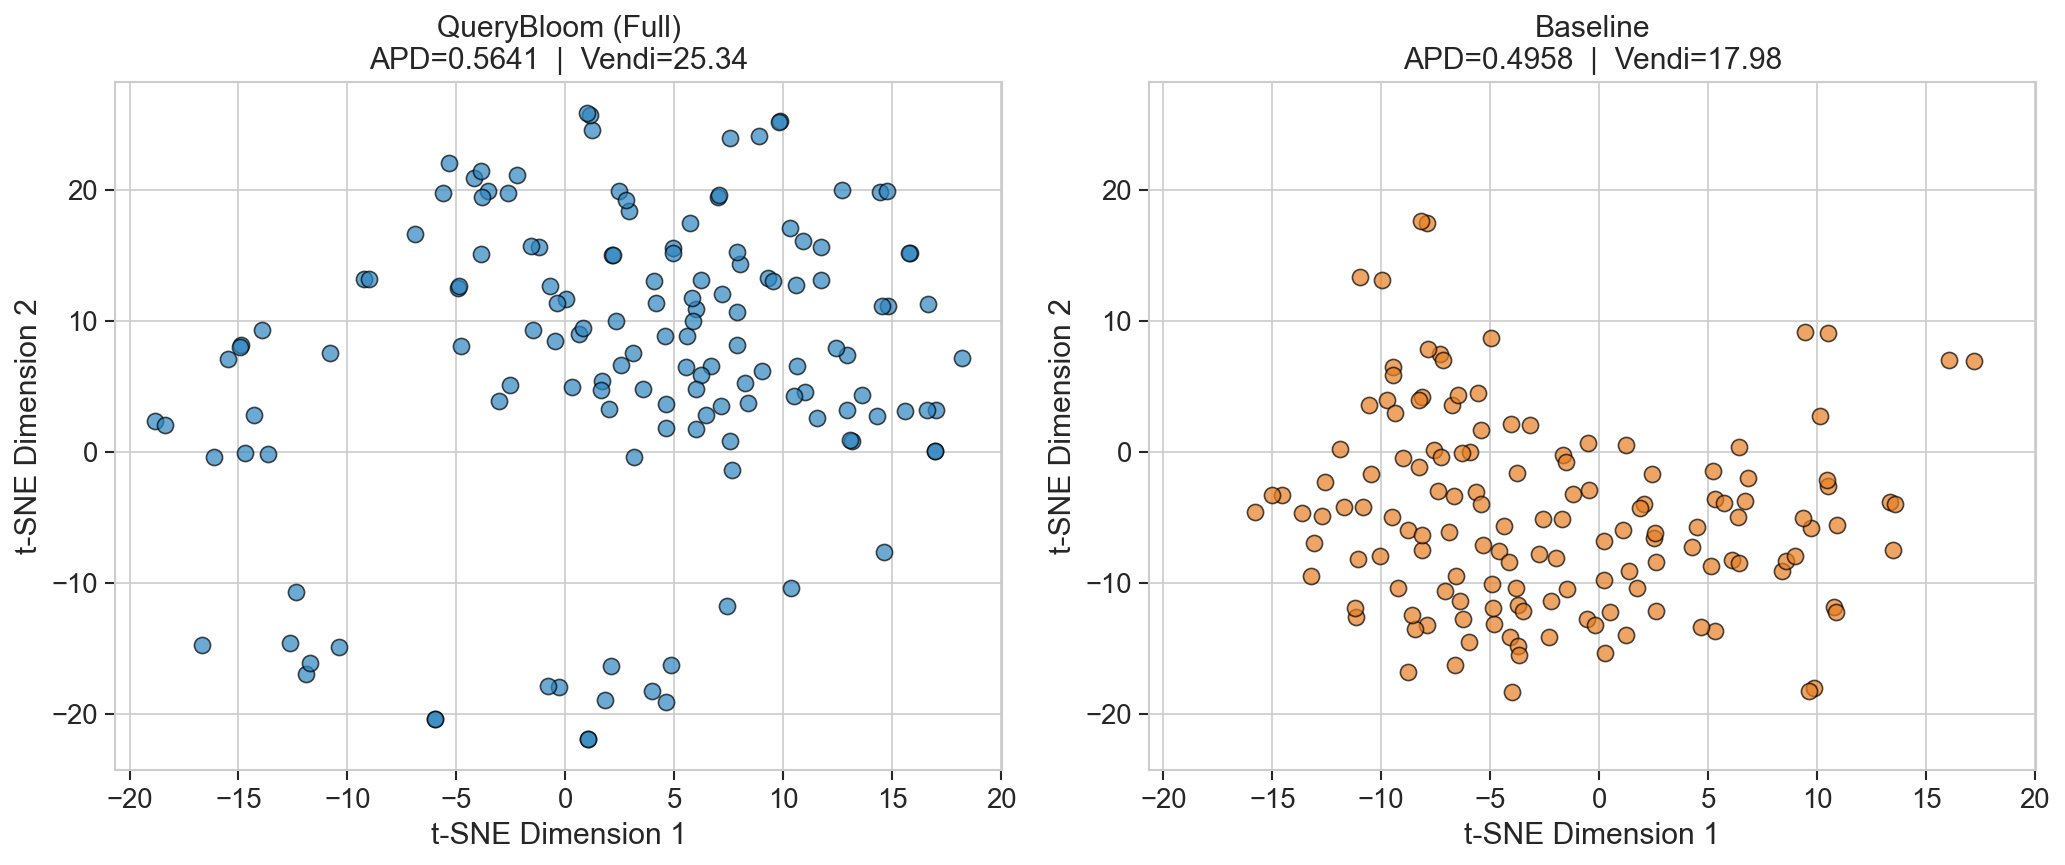
\includegraphics[width=\textwidth]{figures/eval/semantic-dbpedia.png}
    \caption*{DBpedia knowledge graph}
\end{figure*}
\clearpage

\begin{figure*}[p]
    \centering
    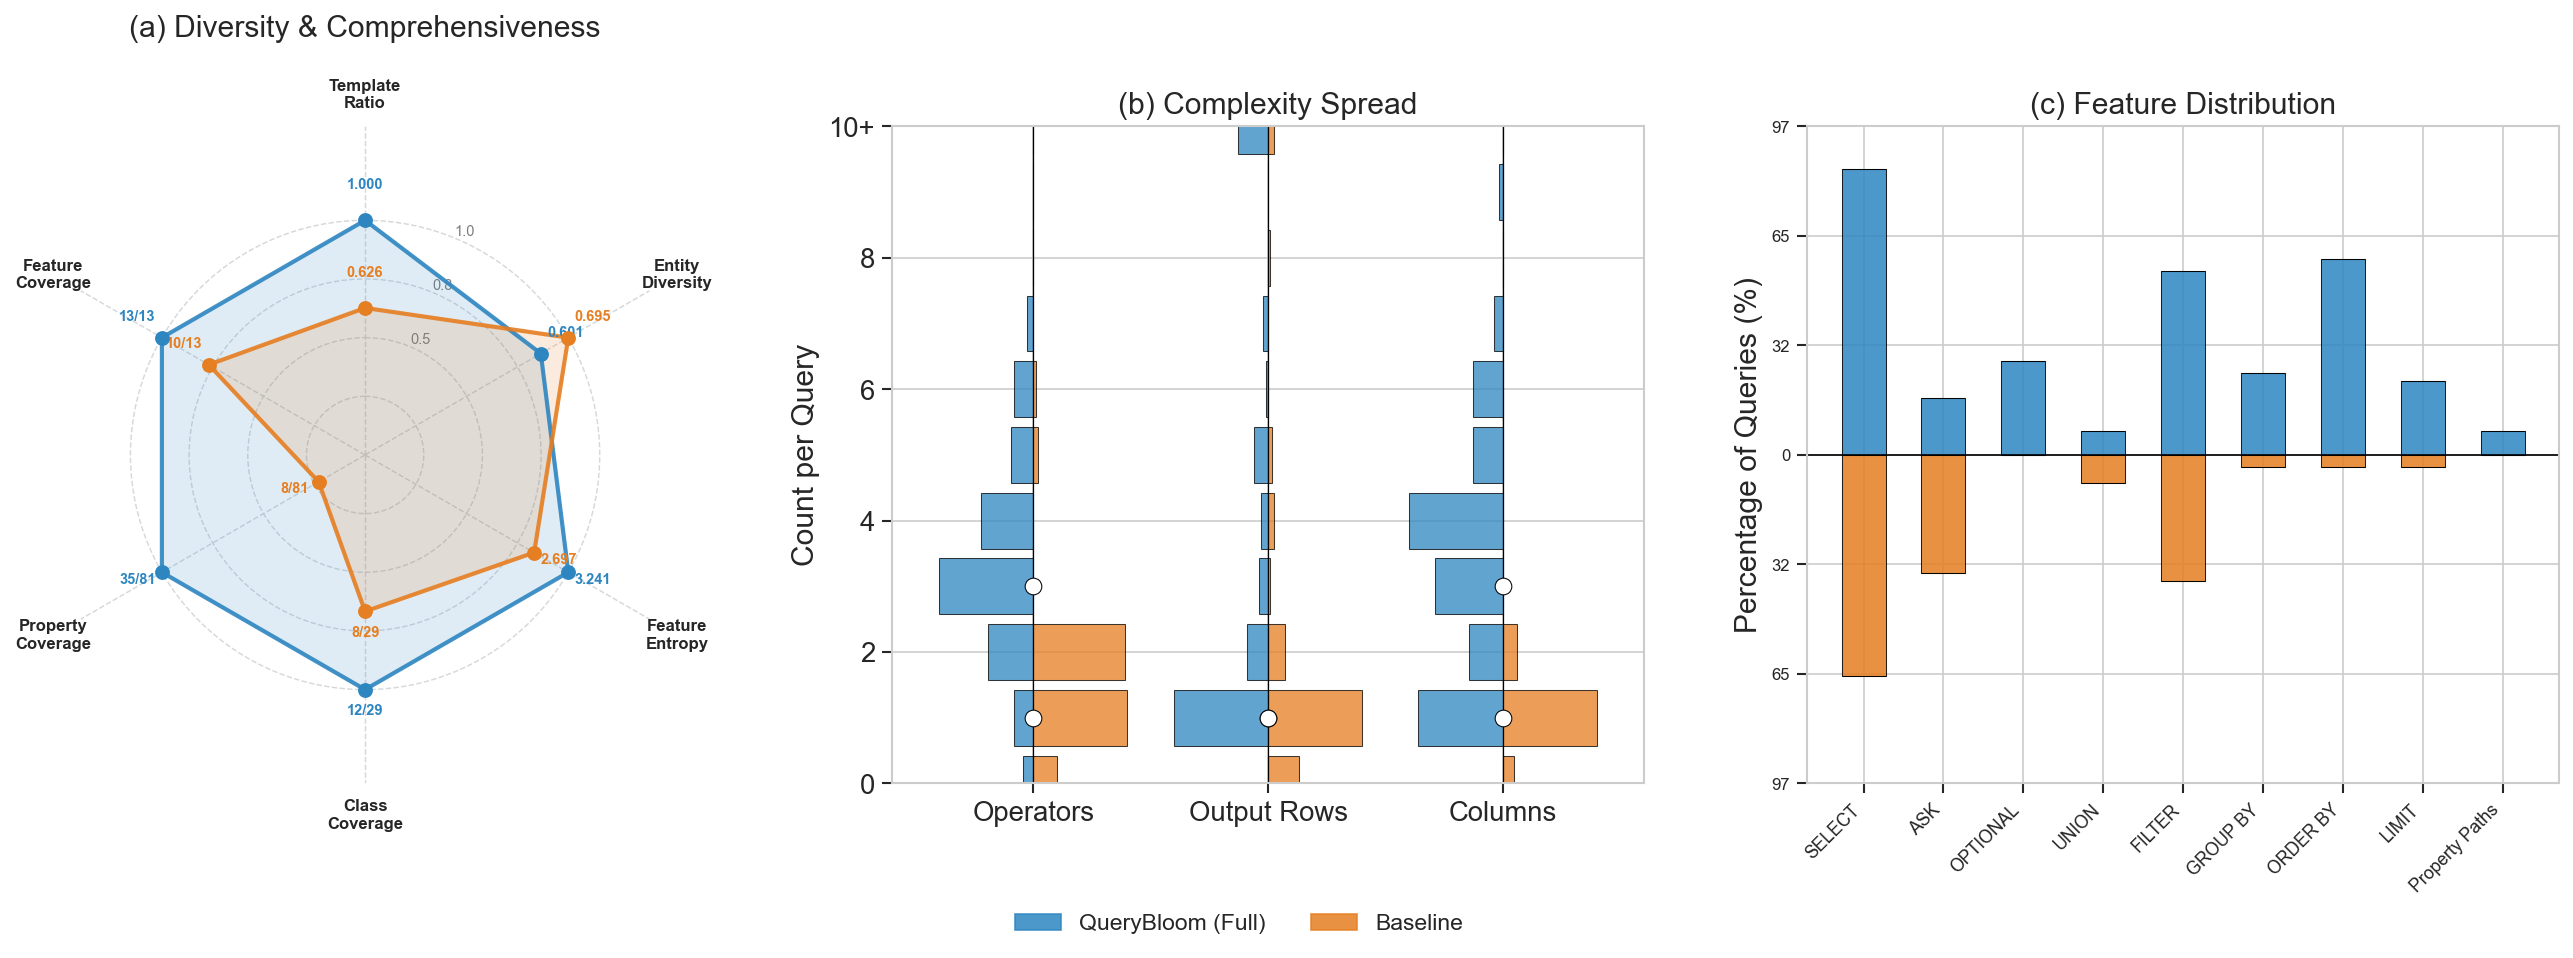
\includegraphics[width=\textwidth]{figures/eval/diversity-dblp.png}
    \par\medskip
    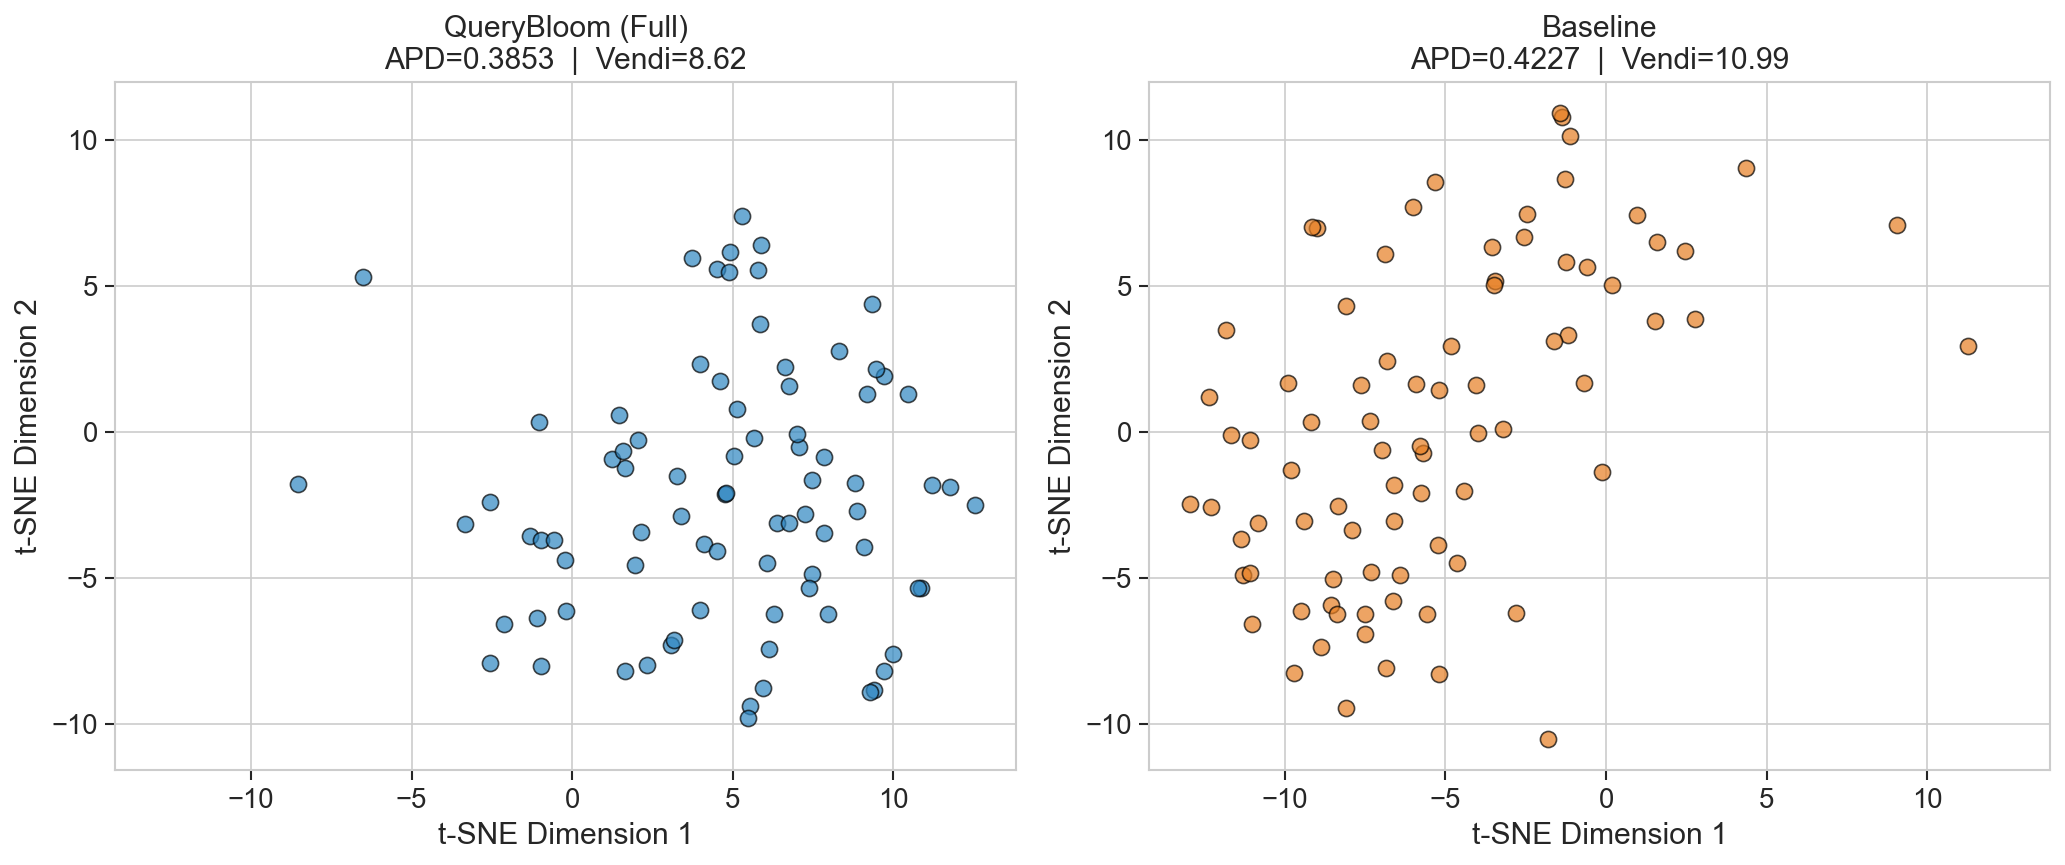
\includegraphics[width=\textwidth]{figures/eval/semantic-dblp.png}
    \caption*{DBLP knowledge graph}
\end{figure*}

\clearpage
\section{Conclusion}

We presented QueryBloom, a KG-agnostic methodology for automatically synthesizing diverse, high-quality Text-SPARQL example sets from arbitrary RDF knowledge graphs, requiring only SPARQL endpoint access. Through multi-hop subgraph sampling and LLM-driven verbalization with execution-based verification, QueryBloom produces example sets that match or exceed the diversity of established human-authored benchmarks across query structural complexity, semantic linguistic variety, and schema coverage. By addressing the example scarcity challenge for domain-specific knowledge graphs, QueryBloom can support the development and evaluation of KGQA systems in specialized domains where curated resources are unavailable, while also serving as executable documentation that helps practitioners understand unfamiliar graph structures.

\clearpage
\bibliography{references}

\onecolumn
\appendix
\section{Prompts}
\label{sec:appendix_prompt}
\subsection{QueryBloom Generation Prompt}
\label{sec:appendix_prompt_generate}
\begin{tcblisting}{
  colback=blue!5!white,
  colframe=blue!75!black,
  title=Structure of the Generation Prompt,
  breakable,
  listing only,
  listing options={basicstyle=\ttfamily\scriptsize,breaklines=true,columns=fullflexible}
}
You are an expert in analyzing a subgraph sampled from a knowledge graph and generating natural language questions with corresponding SPARQL
queries.


{% if kg_title %}
**Knowledge Graph Title:** {{ kg_title }}
{% endif %}
{% if kg_description %}
**Knowledge Graph Description:** {{ kg_description }}
{% endif %}

Given the following subgraph description loaded from a YAML file, generate
natural language questions that could be answered by querying the full knowledge graph, along with their corresponding
SPARQL queries.

### YAML Subgraph Description:
<Subgraph>
    {{ subgraph_pattern }}
</Subgraph>

Notes on the YAML structure (generic, do not assume any specific KG):
- Each subgraph includes: subgraph_id, num_types, min_support, types, edges, predicate_uris.
- types is a mapping from type label to:
- uri (class URI)
- sample_entities (a few example entity URIs, sometimes with attributes shown as a compact string like attr:type=value)
- edges is a list of triples in a readable form: "TypeA --predicateLabel --> TypeB".
- if an edge ends with "\*" after the arrow, it denotes an optional property (after adding the edge, the graph doesn't
meet the support property).
- predicate_uris lists predicate URIs aligned with the edges.
- Attributes marked with "\*" are below the subgraph's support threshold (optional attributes).

### Task:
First, assess whether this subgraph allows for meaningful questions. If the subgraph is too trivial, lacks interesting
relationships (eg, graph metadata as opposed to actual knowledge), or doesn't support generating useful and meaningful questions, set is_meaningful to false and return an empty questions
list.

If is_meaningful is true, generate 2-4 question-query pairs as a JSON array where each item has:
- text_query: the natural language question
- sparql_query: the corresponding SPARQL query



### Requirements:
1. Generate 2-4 question-query pairs depending on your assessment of the subgraph's richness. Try to attain high coverage of all the meaningful aspects of the subgraph in the question-query pairs.
2. Questions should be grounded in the classes, entities, relationships and attributes in this YAML subgraph. Using classes, entities, relationships and attributes not in the YAML subgraph is strictly prohibited!
3. Do not reference the YAML or the subgraph itself in the natural language question (each of text and query should be self-contained) and never mention a URI/prefix in the text question (or use knowledge graph terminology like properties, types, etc.)
4. Questions should be certaintly answerable and avoid ontology/schema/documentation questions
5. Focus on questions that are interesting and meaningful (avoid meaningless questions like "what/how many entities are linked to.../useless patterns...")
{% if focus_entity_qa %}
6. Great questions are often centered around interesting entities in the graph. All of the questions you produce must be entity centric.
Meanwhile, set is_meaningful to False if no interesting entities are available.
7. Make questions diverse in style (what, who, whom, whose, when, which, yes/no questions, how compounds, statistics, etc.) and complexity but while maintaining the quality of the questions and meaningfulness
{% else %}
6. Whenever there is an interesting entity is in the graph, it's good to have a question or two specifically about it
7. Make questions diverse in style (SELECT, SELECT + AGGREGATION, ASK, as appropriate) and complexity (MIN/MAX/AVG/COUNT/SUM, GROUP BY/FILTER/HAVING, EXISTS/OPTIONAL, nesting, etc.) but while maintaining the quality of the questions and meaningfulness
{% endif %}
8. Declare meaningful prefixes in the query based on the URIs in the yaml
9. Use proper SPARQL syntax to generate valid queries. Your sparql query must produce exactly the results expected by the text query.
10. If the question does not have one answer/result, you may or may not use LIMIT in SELECT queries (e.g., LIMIT 100) to avoid too many results. BUT MAKE SURE to REFLECT THIS in the text query!
11. SPARQL queries should be stand-alone executable against a SPARQL endpoint containing the full graph
12. If a term is awkward in the graph, and you are confident it can be rephrased naturally without being inaccurate, do so
13. The phrasing of the natural language question should be always natural, fluent and not awkward or stilted. Question should always end with a question mark.

### Final Note:
The ultimate goal is to produce high-quality, diverse, and very meaningful questions together with their corresponding
accurate SPARQL queries that can be executed against the full knowledge graph.

Another essential property is that an expert in the knowledge graph should be able to reproduce the same sparql query when given text question only.
- You will be penalized if the generated SPARQL query and the text question do not properly align (eg, the sparql query has constraints unrequested in the question... or misses requested ones)
- You will be also highly penalized if the generated SPARQL query incorrectly answer the text question or provides no answer when there is one.
- You will be penalized if your question styles are not diverse enough, if questions are of low quality or are phrased awkwardly.
- You will be rewarded when you generate questions an expert in the domain would ask where the sparql query being perfectly aligned to the question and accurately answering it. 
- Flagging the subgraph as not meaningful when it's hard to generate high quality questions is better than generating low quality questions.
- Generating fewer high quality questions that a DOMAIN EXPERT may ask is MUCH better than generating more low quality questions. Quality over quantity.
\end{tcblisting}


\subsection{QueryBloom Verification Prompt}
\label{sec:appendix_prompt_verify}
\begin{tcblisting}{
  colback=orange!5!white,
  colframe=orange!75!black,
  title=Verification Prompt for Question--Query Pairs,
  breakable,
  listing only,
  listing options={basicstyle=\ttfamily\scriptsize,breaklines=true,columns=fullflexible}
}
You are an expert in SPARQL and knowledge graph querying. You are reviewing question-query pairs that were generated
from a subgraph pattern and then executed against a SPARQL endpoint.

Your task is to verify whether each question-query pair is correct based on the execution results.

### Original Subgraph Pattern:
<Subgraph>
    {{ subgraph_pattern }}
</Subgraph>

### Generated Question-Query Pairs with Execution Results:
{% for qa in qa_pairs %}
**Pair {{ loop.index }}:**
- **Question:** {{ qa.question }}
- **SPARQL Query:**
```sparql
{{ qa.sparql_query }}
```
- **Execution Success:** {{ qa.execution_results.success }}
- **Result Count:** {{ qa.execution_results.count }}
{% if qa.execution_results.error_message %}- **Error:** {{ qa.execution_results.error_message }}{% endif %}
{% if qa.execution_results.result_preview %}- **Result Preview (first 3 rows):** {{ qa.execution_results.result_preview
}}{% endif %}

{% endfor %}

### Task:
For each question-query pair, assess whether it is **correct**, **needs_fix**, or **unfixable** based on:
1. Did the SPARQL query execute successfully?
2. Does the query correctly answer the natural language question? Are they consistent?
3. Are there any necessary fixes to the text or sparql queries.

Set `all_correct` to true only if ALL pairs are correct. If ANY pair needs fixing, set `all_correct` to false.

For pairs that need fixing:
- Provide a brief explanation in `reason`
- Provide the corrected question in `fixed_text_query`
- Provide the corrected SPARQL query in `fixed_sparql_query`

For correct pairs, leave `fixed_text_query` and `fixed_sparql_query` as null.

**Important:** a query that errors out, returns no results when it should, or doesn't match the question
semantics should be marked as `needs_fix`. Use `unfixable` only when no reliable correction exists.
\end{tcblisting}


\end{document}
